\sujet{Geometry}

\noindent
Durée : 1h30 - 20 points\\


\section{Geometrical characterization}
\index{Characterization}

\begin{figure}[htbp]
 \centering
 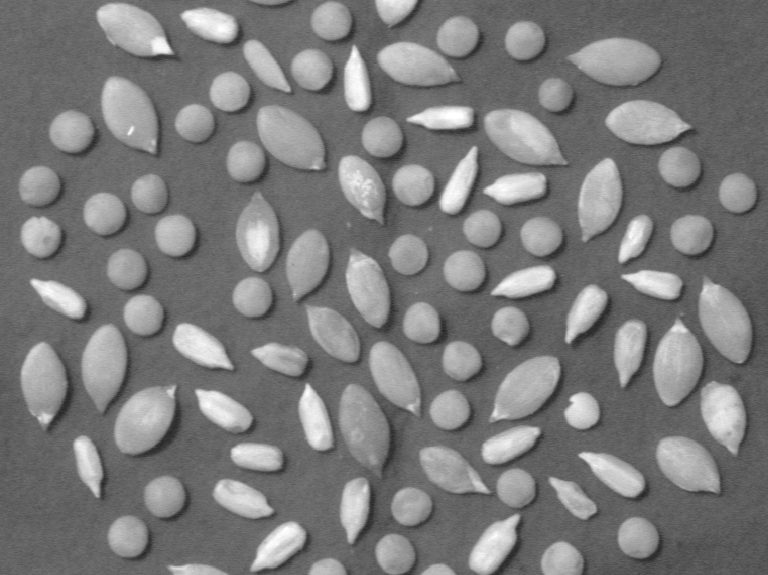
\includegraphics[width=8cm]{seeds.png}
 
\includegraphics[width=8cm]{segmentation.png}
 \caption{This image contains grains with different shapes. 3 different types of grains can be observed. An idea of the segmentation result is proposed.}
 \label{fig:exam_2016:seeds}
\end{figure}

\begin{qbox}
With the grayscale image of Fig.\ref{fig:exam_2016:seeds}, propose a method to count the number of grains of each type.
\end{qbox}

\begin{mcomment}
\begin{mremark}
The function \minline{ind2rgb} can convert a labelled array into a RGB image with the following syntax: \minline{ind2rgb(L, lines(4));}, 
with \minline{lines(4)} defining a colormap with 4 colors. It has been used to generate the segmented image.
\end{mremark}
\end{mcomment}

\section{Stochastic geometry}
\index{Spatial Processes}

Let $X$ be a random set defined as a rectangle with sides $a, b$ and an orientation $\theta$ in relation to the $x$-axis. $a$ and $b$ are independant random variables. $a$ follows a Normal law with parameters $(\mu_a,\sigma_a)$. $b$ follows a Normal law with parameters $(\mu_b,\sigma_b)$.  $\theta$ follows a uniform distribution between $0$ and $2\pi$.

\begin{qbox}
\begin{itemize}
\item Show different realizations of the random set $X$ with the parameters $\mu_a=50, \sigma_a=10,\mu_b=100,\sigma_b=30$.
\item Calculate (from an analytical point of view) the expectation of the area and of the squared area of this random set, denoted $\mathbb{E}[A(X)]$ and $\mathbb{E}[A^2(X)]$ respectively, as a function of $\mu_a,\mu_b,\sigma_a,\sigma_b$.
\item From $N=1000$ realizations of this random set (using the parameters given in question 1), compute $\mathbb{E}[A(X)]$ and $\mathbb{E}[A^2(X)]$. Deduce and compare the estimated parameters of the Normal laws to the real ones.
\item Show (in a graph) the resulting error of the estimation as a function of the number of realizations $N$. 
\end{itemize}
\end{qbox}

\begin{mcomment}
\begin{mremark}
You can use the Matlab function \minline{randn} to generate some realizations of a Normal distribution.
\end{mremark}
\end{mcomment}
